%%
%% 研究報告用スイッチ
%% [techrep]
%%
%% 欧文表記無しのスイッチ(etitle,eabstractは任意)
%% [noauthor]
%%

%\documentclass[submit,techrep]{ipsj}
%%% <<< SES
%\documentclass[submit,techrep,noauthor]{ipsj}
\documentclass[submit,ses,noauthor]{ipsj}
%%% >>> SES


%\usepackage[dvips]{graphicx}
\usepackage[dvipdfmx]{graphicx}
\usepackage{latexsym}
\usepackage[T1]{fontenc}
\usepackage{lmodern}
\usepackage{textcomp}
\usepackage{latexsym}
\usepackage{url}
\usepackage[noadjust]{cite}
%\usepackage[fleqn]{amsmath}
%\usepackage{amssymb}
\usepackage{listings}
%\usepackage{jlisting}
\usepackage{ascmac}
%\usepackage{fancybx}

\newcommand{\todo}[1]{\colorbox{yellow}{{\bf TODO}:}{\color{red} {\textbf{[#1]}}}}

\def\Underline{\setbox0\hbox\bgroup\let\\\endUnderline}
\def\endUnderline{\vphantom{y}\egroup\smash{\underline{\box0}}\\}
\def\|{\verb|}
%

%\setcounter{巻数}{59}%vol59=2018
%\setcounter{号数}{10}
%\setcounter{page}{1}


\begin{document}


\title{バージョンに導入される変更提案の特徴分析}

\etitle{How to Prepare Your Paper for IPSJ SIG Technical Report \\ (version 2018/10/29)}

\affiliate{WA}{和歌山大学\\
Faculty of Systems Engineering, Wakayama University, 30 Sakaedani, Wakayama, 640--8441 Japan}


\paffiliate{NAIST}{奈良先端科学技術大学院大学\\
Nara Institute of Science and Technology, 8916--5 Takayama-cho, Ikoma, Nara, 630--0192 Japan}

\author{上中 瑞稀}{Uenaka Mizuki}{WA}[s246035@wakayama-u.ac.jp]
\author{伊原 彰紀}{Ihara Akinori}{WA}[ihara@wakayama-u.ac.jp]
\author{柏 祐太郎}{Kashiwa Yutaro}{NAIST}[yutaro.kashiwa@is.naist.jp]

\begin{abstract}
\todo{SSのまま}大規模なプロジェクトには,ソースコードの変更提案が日々膨大に提出される.プロジェクトの開発者は,ソースコードの品質や保守性の向上のために変更提案を順に検証するが,検証が遅延する変更提案が少なくない.本研究では,直近のバージョンで導入される変更提案を優先的に選択するために,リリースまでの期間に導入される変更提案同士の特徴の違いを明らかにした後,直近のバージョンで導入される変更提案の選択手法を提案する.具体的には,個々の変更提案の特徴を機械学習アルゴリズムに学習したモデルにより,リリースまでの期間に応じた変更提案の予測精度,および予測に寄与する特徴を比較した.分析の結果,リリースまでの期間に応じて変更提案の選択に重要となる特徴が変化することを確かめた.
\end{abstract}


%
%\begin{jkeyword}
%情報処理学会論文誌ジャーナル,\LaTeX,スタイルファイル,べからず集
%\end{jkeyword}
%
%\begin{eabstract}
%This document is a guide to prepare a draft for submitting to IPSJ
%Journal, and the final camera-ready manuscript of a paper to appear in
%IPSJ Journal, using {\LaTeX} and special style files.  Since this
%document itself is produced with the style files, it will help you to
%refer its source file which is distributed with the style files.
%\end{eabstract}
%
%\begin{ekeyword}
%IPSJ Journal, \LaTeX, style files, ``Dos and Dont's'' list
%\end{ekeyword}

\maketitle

%%%%%%%%%%%%%%%%
\section{はじめに}
%%%%%%%%%%%%%%%%

ソフトウェア開発において,変更提案されたソースコードの可読性や欠陥の有無を開発者が評価するコードレビューの作業は,ソフトウェアの品質維持のために重要な役割を担っている~\cite{quality1}\cite{quality2}.コードレビューでは,高品質なソフトウェアをリリースするために,複数人の開発者(検証者)がソースコードを検証し,ソースコードを実装した開発者(実装者)とソースコード変更の妥当性の合意形成を図り,必要に応じて修正を繰り返す.コードレビューは,ソフトウェア開発プロセスの一連の作業において,時間,作業量ともに高いコストを要する作業となっている\cite{}.
%The economics of software quality assurance: A simulation based case study. を引用

コードレビューを効率化するため,昨今では多くのソフトウェア開発においてGitHub,Gerrit,Review Boardなどのオンラインコードレビューサービスを利用したコードレビュー方式(モダンコードレビュー\cite{})を導入している.\todo{どの程度効率化したか引用がほしい.}
%Alberto Bacchelli and Christian Bird. Expectations, outcomes, and challenges of modern code review. In Proc. ICSE’13, pp. 712\UTF{2013}721
この方式を導入しているプロジェクトであっても,日々膨大なソースコードの変更提案が提出される大規模なプロジェクトでは,検証者がコードレビューに数日かかることも少なくない\cite{}.
%引用ほしい
検証者は直近にリリースするバージョンに導入する変更提案としてソフトウェアの脆弱性を解決する変更提案などを優先して検証する.\todo{}
%引用ほしい

従来研究では,機械学習アルゴリズムを用いて個々の変更提案の特徴(\todo{XやXなど})に基づき,変更提案が翌日までに検証する変更提案を推薦する手法を提案している\cite{prioritizer}.この従来研究では,個々の変更提案に対する開発者の関心,変更提案をソフトウェアに適用する難しさなどを捉えるモデルを開発し,\todo{XX}への有用性を示している.しかし,従来研究の手法では\todo{XX}のような変更提案については精度が低い.その理由として,予測時点における未対応の変更提案数,対応可能な開発者数,直近のリリースまでの期間などの開発状況によって,検証する変更提案の優先順位は異なることが示唆される.\cite{}
%引用欲しい
開発状況に応じて優先的に検証すべき変更提案を明らかにすることで,直近にリリースするバージョンに含める変更提案の検証,および効率的な開発計画の立案を支援できると考える.
%この研究によって,機能間の関係性も考えて検証する,修正する変更提案の順番の研究もできそう.

本論文では,直近のリリースまでの期間に応じた変更提案の特徴の違いを明らかにする.さらに,優先的に検証することが期待される変更提案の中から,限られた開発リソースで検証可能な変更提案を明らかにし,実際に検証された変更提案との違いを分析する.本論文では3つの調査質問に対して分析を行う.

\noindent\textbf{RQ1: リリースまでの期間に応じた変更提案の特徴は異なるのか?}\\
RQ1(3章)では,リリースまでの期間に応じて検証されている変更提案の特徴量を比較する.特徴量は,従来研究で提案されている個々の変更提案の特徴(X種類)に加え,リリースまでの期間に応じた開発状況を捉えるための特徴(X種類)を計測する.

\noindent\textbf{RQ2: 変更提案の特徴に基づき,直近のリリースに導入される変更提案をどの程度予測できるのか?}\\
RQ2(4章)では,RQ1で計測した特徴量を用いて,直近にリリースされるバージョンに導入する変更提案を予測する機械学習モデルを構築する.

\noindent\textbf{RQ3: 優先的に検証される特徴を持つ変更提案のうち,開発者が検証可能と示唆される変更提案は価値があるのか?\todo{難w}}\\
RQ3(5章)では,ナップサック問題を用いて特定の時期において検証可能と示唆される変更提案を選択し,実際に検証される変更提案と比較する.具体的には,特定の時期において開発者が検証可能なソースコード行数を上限とし,RQ2で推薦される変更提案の変更行数の加算がその上限に達するまでを検証可能な変更提案として選択する.

以降,本論文では,\ref{chap:intro}章でOSS開発におけるコードレビュープロセスと従来研究について述べる.その後,\ref{chap:dataset}章で本論文で対象とするデータセット,および,RQ1の分析手法と結果を述べる.\ref{chap:rq-1}章と\ref{chap:rq-2}章でそれぞれRQ2,RQ3の手法と結果を述べる.そして,\ref{chap:disc}章で結果の考察および妥当性について述べ,\ref{chap:fig-tab-exp}章でまとめる.

%%%%%%%%%%%%%%%%
\section{ソフトウェア開発におけるコードレビュープロセス}\label{chap:intro}
%%%%%%%%%%%%%%%%

\subsection{コードレビュープロセス}

%ソフトウェア開発において,開発者は,不具合修正や機能追加のために変更したソースコードの内容を変更提案としてプロジェクトに提出する.プロジェクトのレビュアーは,提出された変更提案に対して,ソースコードの可読性や欠陥の有無といったソースコードの品質を評価するコードレビューという開発プロセスを行うことで,ソースコードの一貫性や保守性を維持している.コードレビューにおいて,レビュアーは変更提案に対して,プロジェクトに導入する必要があるか否か,プロジェクトに導入可能な水準に達しているか否かを判断する.
図\ref{fig:codereviewprocess}はコードレビュープロセスの流れを説明する概略図を示す.検証者はコードレビューに基づく判断によって,変更提案に対して,修正要求,導入,却下のいずれかを判断する.修正要求は,変更提案を提出した実装者に,検証した結果を伝えソースコードの改修を依頼する.この作業を繰り返すことで,ソフトウェアの品質を維持しつつ,不具合修正やさらなる機能拡張を行う.

コードレビューはソフトウェア開発に多大な貢献をもたらす一方で,膨大なコストがかかる作業でもある.1つの変更提案に数日から数ヶ月の期間を要することもあり,1週間で平均6時間程度をコードレビューに費やす\cite{review2}.特に,オープンソースソフトウェア開発では,不特定多数の開発者が変更提案を提出するため,日々膨大な変更提案が提出される.従って,検証者は直近にリリースするバージョンに導入する変更提案としてソフトウェアの脆弱性を解決する変更提案などを優先して検証する.\cite{}

%膨大な変更提案全てに対してコードレビューを行うことは困難であるため,コードレビュー対象とする変更提案を選択する必要があるが,コードレビューする変更提案の選択もまた,変更提案が膨大であるため容易ではない.

%-----------------------
\begin{figure}[t]
\begin{center}
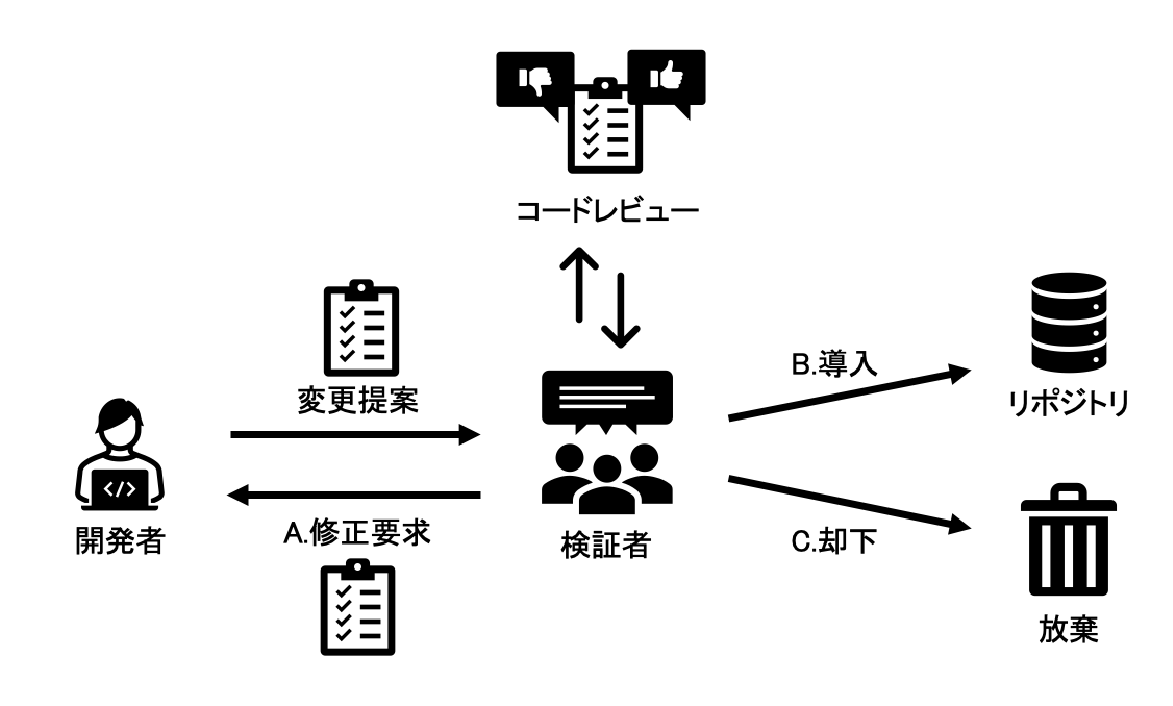
\includegraphics[width=1.0\linewidth]{fig/CodeReviewProcess.eps}
\caption{コードレビュープロセス\todo{開発者は実装者,ABCは削除}}
\label{fig:codereviewprocess}
\end{center}
\end{figure}
%-----------------------

\todo{ここまでチェック済み}


\subsection{従来研究}

\subsubsection{変更提案の優先順位付け}
従来研究では,OSS開発における,コードレビューを行う変更提案の選択が困難であるという課題を解決するために,変更提案の優先順位付けの手法を提案している.従来研究では,説明変数として表\ref{table:juurai}に示す変更内容や作成者の特徴などの変更提案の14種類の特徴と,目的変数として翌日までにコメントやコードレビューされるか否かを機械学習アルゴリズム(ランダムフォレスト)に学習させ,学習させた機械学習モデルを用いて,各変更提案が翌日にレビューされる確率に基づいて変更提案の優先順位を予測している\cite{prioritizer}.機械学習モデルの性能評価のために,475プロジェクトに対して10分割交差検証を10回ずつ行った結果,適合率0.64,再現率0.85を達成している.

%\begin{table}[t]
%  \caption{従来研究\cite{prioritizer}で用いる14種類の説明変数}
%  \label{table:juurai}
%  \centering
%  \vspace{0.5zh}
%  \begin{tabular}{l|lr}
%    \hline
%    \multicolumn{1}{c|}{説明変数}  & \multicolumn{1}{|c}{説明}  \\
%    \hline \hline
%    経過時間  & 変更提案が提出されてからの経過分数 \\
%    貢献率  & 変更提案作成者のプロジェクトでのコミット率 \\
%    受入率  & 変更提案作成者が過去に提出した変更提案の導入率 \\
%    追加行数  &  変更提案で追加されている変更行数 \\
%    削除行数  & 変更提案で削除されている変更行数  \\
%    リビジョン数  & 変更提案のリビジョン数 \\
%    ファイル数  & 変更提案の変更ファイル数 \\
%    コメント数 & 変更提案のコメント数 \\
%    レビュー数  &  変更提案に対してのコードレビュー数 \\
%    コアメンバー  & 変更提案の作者はプロジェクトメンバーか \\
%    ブランチ  & 変更コードとマージ先のリポジトリが同一か \\
%    issue含有  & 変更提案に紐づいているissueがあるか \\
%    最終コメント &  最終コメントでユーザがメンションされているか \\
%    テストコード含有  & 変更ファイルにテストコードが含まれているか \\
%    \hline
%  \end{tabular}
%\end{table}


\subsubsection{変更提案の導入と開発者間の関係}
Bosu\cite{review1}らは,OSS開発における開発者の地位が変更提案の導入に影響するのか否かを明らかにするために,OSS開発を活発に行う開発者と不活発な開発者での変更提案の導入プロセスの違いに関する調査を行なった.8つのOSSプロジェクトから導入もしくは却下と判断された変更提案のコードレビューデータを調査した結果,OSS開発を活発に行う開発者の方が,不活発な開発者より変更提案の導入率が高いことが明らかとなった.また,OSS開発を活発に行う開発者の方が,変更提案に対して初回のコードレビューが行われる時間が短いことや,変更提案に対して初回のコードレビューが行われてから,導入もしくは却下の判断が為されるまでの時間が短いことも明らかとなった.そのため本研究では,開発で導入される変更提案の予測モデル構築の際に,初回のコードレビューが行われるまでの時間や,初回のコードレビューが行われてからの時間を特徴量として学習させることで,予測精度の向上を図る.


\subsection{動機}
従来研究\cite{prioritizer}では,ソフトウェア開発において優先的にコードレビューを行う変更提案の選択を容易にするために,変更提案に対して優先順位付けを行なっているが,変更提案の特徴量のみを用いて予測を行うため,直近のバージョンリリースまでの期間やその時点での対応可能な開発者数などの開発状況は考慮されていない.しかし,ソフトウェア開発において,バージョンリリースが近い場合は新たに提出された大規模な変更を導入するためにコードレビューのリソースを割く時間が無いというように,開発状況によって対応する変更提案は異なると考える.RQでは,リリースまでの期間に応じた変更提案の導入に重要な特徴を調査する.

\section{リサーチクエスチョン}
本論文では,2つのRQを設定し,検証することで本研究の選択手法が直近のバージョンリリースに導入される変更提案の選択に有効かを評価する.
 \begin{itemize}
  \item RQ1:リリースまでの期間に応じて優先的に導入される変更提案の特徴は異なるか?
  \item RQ2:開発状況を考慮した変更提案の選択手法は直近のバージョンリリースに導入される変更提案をどの程度選択するか?
 \end{itemize}
 
 RQ1では,リリースまでの期間に応じた変更提案の導入に重要な特徴の調査を行う.RQ2では,ナップサック問題を用いて変更提案の選択手法を定式化し,実際に行われた開発と比較することで,実際の開発で導入された変更提案をどの程度選択するかの調査を行う.
 
 
%%%%%%%%%%%%%%%%
\section{分析対象データセット}\label{chap:dataset}
%%%%%%%%%%%%%%%%

本章では,RQに共通して用いるデータセットを説明する.本論文では,OpenStackにおけるプロジェクトの中から,導入もしくは却下と判断された変更提案が多いNeutron,Keystone,Horizon,Novaプロジェクトを分析対象プロジェクトとし,各プロジェクトの変更提案の中から,収集時点で導入もしくは却下されることが決定している変更提案を,各リビジョンごとに収集する.具体的には,コードレビュー管理システムであるGerrit\footnote{\url{https://review.opendev.org}}から,それぞれの変更提案のリビジョンごとの特徴量や,コードレビュー履歴を収集し,リポジトリホスティングサービスであるGitHub\footnote{\url{https://github.co.jp/}}から,プロジェクトのコミット履歴や,リリースバージョンのリリース日やコミットハッシュを収集した.4プロジェクトそれぞれの変更提案数は表\ref{table:release}のプロジェクト名の下に示す.また,表\ref{table:release}には,各プロジェクトにおいてリリースされたバージョンと,導入された変更提案数の上位15バージョンを示す.正解ラベルのついた変更提案数を一定以上確保するためにこれら15バージョンを分析対象とする.

%\begin{table}[t]
%\centering
%  \caption{プロジェクトごとの変更提案数}
%  \vspace{0.5zh}
%  \label{table:henkou}
%  \begin{tabular}{l|r}  \hline
%    \multicolumn{1}{c|}{プロジェクト} & \multicolumn{1}{|c}{変更提案数} \\ \hline \hline
%    Neutron & 24,467 \\ \hline
%    Keystone & 10,764 \\ \hline
%    Horizon & 12,475 \\ \hline
%    Nova & 39,870 \\ \hline
%  \end{tabular}
%\end{table}

\begin{table}[t]
\centering
  \caption{プロジェクトごとの対象リリースバージョン}
  \vspace{0.5zh}
  \label{table:release}
  \scalebox{0.75}{
  \begin{tabular}{l|ll|c}  \hline
    \multicolumn{1}{c|}{プロジェクト} & \multicolumn{1}{|c}{リリースバージョン(変更提案数 )}\\ \hline \hline
    Neutron  & 2013.1.g3(317),2013.2.b2(580),2013.2.rc1(423),2014.2.b1(320),\\ 
   (24,467) 	& 2015.1.0b1(391),2015.1.0b2(306),7.0.0.0b1(371),7.0.0.0b3(396),\\ 
	& 8.0.0.0b1(408),8.0.0.0b2(326),9.0.0.0b3(363),11.0.0.0b3(388),\\ 
	& 15.0.0.0b1(312),19.0.0.0rc1(420),20.0.0.0rc1(380) \\ \hline
    Keystone  & 2011.3(195),essex-4(357),2013.2.b1(186),2013.2.b3(261),\\
    (10,764) & 2014.1.b3(252),2014.2.b1(185),2015.1.0rc1(199),8.0.0a0(187),\\ 
     & 9.0.0.0b2(212),9.0.0.0b3(214),10.0.0.0b1(179),10.0.0.0b2(220),\\ 
     & 11.0.0.0b1(273),15.0.0.0rc1(408),16.0.0.0rc1(225) \\ \hline
    Horizon  & folsom-2(391),2014.2.b2(190),2014.2.b3(279),2015.1.0b2(198),\\
    (12,475) & 2015.1.0b3(237),8.0.0.0b2(402),8.0.0.0b3(384),9.0.0.0b1(230),\\
      & 9.0.0.0b3(237),10.0.0.0b2(193),10.0.0.0b3(171),11.0.0.0b2(193),\\
       & 13.0.0.0b1(310),14.0.0.0b1(194),15.0.0.0b2(178) \\ \hline
    Nova & folsom-1(1,550),2013.1.rc1(2723),2013.2.b3(1,517),2013.2.rc1(555),\\ 
   (39,870)  & 2014.1.b3(517),2014.2.b2(554),2015.1.0b2(838),2015.1.0b3(625),\\
     & 13.0.0.0b3(529),14.0.0.0b2(607),16.0.0.0b2(524),17.0.0.0b1(516),\\ 
     &19.0.0.0rc1(865),21.0.0.0rc1(808),24.0.0.0rc1(771) \\ \hline
  \end{tabular}
  }
\end{table}

%%%%%%%%%%%%%%%%
\section{RQ1: リリースまでの期間に応じて優先的に導入される変更提案の特徴は異なるか?}\label{chap:rq-1}
%%%%%%%%%%%%%%%%

\subsection{概要}
本章では,RQを検証するために,分析対象データセットから変更提案の特徴や変更提案作成者に関する16種類の説明変数と目的変数を計測し,ランダムフォレストを用いて分析対象とするバージョンリリースまでに導入される確率を予測するモデルを構築する.構築した予測モデルを用いて,リリースまでの異なる時点ごとに分析対象とするバージョンリリースまでに導入される変更提案を予測する.異なる時点ごとでの予測精度とそれぞれの説明変数の重要度を比較することで,リリースまでの期間に応じて優先的に導入される変更提案の特徴の違いを明らかにする.

図\ref{fig:RQ1_figure}は分析方法の概略図を示す.本分析では,リリースまでの期間の違いによって優先的に導入される変更提案の特徴が異なるか否かを分析するために,対象リリースバージョンまでの異なる時点に存在する変更提案の特徴量を算出する.また,予測モデルの構築の際は,予測するバージョンより前にリリースされたバージョンのリリースN日前の時点で存在する変更提案を学習データ,予測するバージョンのリリースN日前に存在する変更提案をテストデータとして用いる.

\begin{figure}[t]
\begin{center}
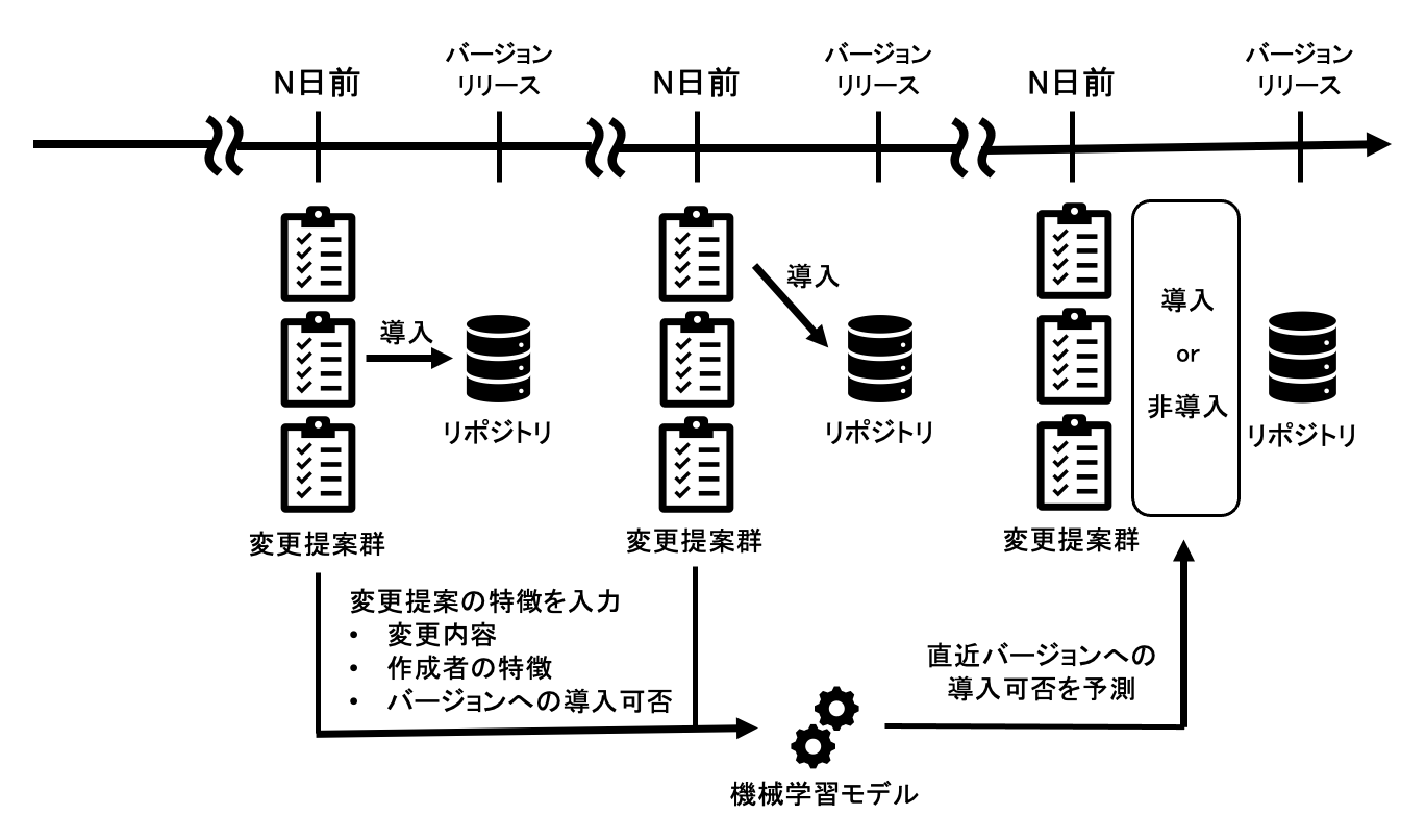
\includegraphics[width=1.0\linewidth]{fig/RQ1_figure.eps}
\caption{RQの分析概略図(リリースN日前を対象とした場合)}
\label{fig:RQ1_figure}
\end{center}
\end{figure}

\subsection{変更提案の導入確率予測モデルの構築}\label{model}
変更提案の導入確率の予測モデルを構築するために,本研究では対象データセットとするプロジェクトの予測時点での変更提案のリビジョンから16種類の説明変数を計測する.表\ref{table:setsumei}は計測する説明変数を示す.また,変更提案のコミット履歴を追跡し,変更提案が導入されたバージョンを分析することで,変更提案が目的のリリースに導入されるか否かの2値を目的変数として計測する.

また,本論文では,予測モデルの構築のための機械学習アルゴリズムとして,決定木を複数組み合わせてモデル構築を行う教師あり機械学習アルゴリズムであるランダムフォレスト\cite{randomforest}を用いる.ランダムフォレストを用いる利点として,アンサンブル学習によって過学習を防ぐことができる点や,特徴量の正規化や標準化の必要がない点が挙げられる.本論文では,ランダムフォレストをPythonのsklearn.ensemble.RandomForestRegressorを用いて実装する.また,実装の際,パラメータは全てデフォルト値を用いる.

\begin{table}[t]
  \caption{予測モデル構築のための説明変数\todo{従来研究で使われていた変数との区別も書く}}
  \label{table:setsumei}
  \centering
  \scalebox{0.75}{
  \begin{tabular}{l|lr}
    \hline
    \multicolumn{1}{c|}{説明変数}  & \multicolumn{1}{|c}{説明}  \\
    \hline \hline
    経過時間  & 変更提案が提出されてからの経過分数 \\
    貢献率  & 変更提案作成者のプロジェクトでのコミット率 \\
    受入率  & 変更提案作成者が過去に提出した変更提案の導入率 \\
    追加行数  &  変更提案で追加されている変更行数 \\
    削除行数  & 変更提案で削除されている変更行数  \\
    リビジョン数  & 変更提案のリビジョン数 \\
    ファイル数  & 変更提案の変更ファイル数 \\
    レビュー数  &  変更提案に対してのコードレビュー数 \\
    プラスレビュー数  & 変更提案に対してのポジティブなコードレビュー数 \\
    マイナスレビュー数  & 変更提案に対してのネガティブなコードレビュー数 \\
    放置時間 & 変更提案が提出されてから最初にレビューされるまでの経過分数 \\
    レビュー経過時間 & 変更提案が最初にレビューされてからの経過分数 \\
    作成済み変更提案数  & 変更提案作成者が過去に提出した変更提案数 \\
    ブランチ変更提案数  &  ブランチに提出されている変更提案数 \\
    テストコード含有  & 変更ファイルにテストコードが含まれているか否か \\
    issue含有  & 変更提案に紐づいているissueがあるか否か \\
    \hline
  \end{tabular}
  }
\end{table}



\subsection{評価方法}

\subsubsection{予測モデルの評価}
本分析では,予測モデルの性能を評価するために,予測モデルの汎化性能の調査によく用いられる交差検証を用いる.交差検証とは,モデル構築の際にデータセットをK個に分割し,分割したデータセットの中からK-1個を訓練データとしてモデルに学習させ,残りの1個をテストデータとしてモデルの評価を行うという工程をK回繰り返し行うことで,より正確な予測モデルの評価を行うための手法である.単純な交差検証の欠点として,データセットに時系列データを用いた場合,未来のデータを学習したモデルを用いて過去のデータを予測することがあるため,予測モデルの汎化性能を正しく評価できないことが挙げられる.そのため,本論文では予測モデルの汎化性能の調査のために,時系列交差検証 (Time Series Split) を用いる.時系列交差検証とは,モデル構築の際にデータセットをK+1個に分割し,K番目の予測では分割したデータセットの中からK番目までのデータを訓練データとしてモデルに学習させ,K+1番目のデータをテストデータとしてモデルの評価を行うという工程をK回繰り返し行うことで,過去のデータを訓練データ,未来のデータをテストデータとして用いた予測モデルの評価を行うための手法である.なお,時系列交差検証ではデータセットを時系列順で並べておく必要があるため,本論文では4プロジェクトの対象リリースバージョンを交互にリリースの古いバージョンから順にデータセットとする.

また,予測モデルの評価指標として,回帰モデルの評価指標としてよく用いられる平均絶対値誤差(MAE),二乗平均平方根誤差(RMSE),決定係数(\(R^{2}\))を用いる.それぞれの本論文における分類精度の説明を以下に示す.

平均絶対値誤差(MAE)とは,全データに対して,直近のバージョンリリースに導入されるか否か(1,0の2値)と直近のバージョンリリースに導入される確率の差の絶対値の平均値を示す.また,MAEは,0に近いほど精度が高いことを表す.

MAEは,データの総数を\(n\),実際の値を\(y_{i}\),予測する確率を\(\hat{y_{i}}\)とすると,(\ref{calculate_MAE})式で表される.
\begin{equation}
\label{calculate_MAE}
 MAE = \frac{1}{n}\sum^{n}_{i=1}|y_{i} - \hat{y_{i}}|
\end{equation}

二乗平均平方根誤差(RMSE)とは,全データに対して,直近のバージョンリリースに導入されるか否か(1,0の2値)と直近のバージョンリリースに導入される確率の差の2乗の平均値に平方根をとった値を示す.また,RMSEは,0に近いほど精度が高いことを表す.

RMSEは,データの総数を\(n\),実際の値を\(y_{i}\),予測する確率を\(\hat{y_{i}}\)とすると,(\ref{calculate_RMSE})式で表される.
\begin{equation}
\label{calculate_RMSE}
RMSE = \sqrt{\frac{1}{n}\sum^{n}_{i=1}(y_{i} - \hat{y_{i}})^{2}}
\end{equation}

決定係数(\(R^{2}\))とは,データに対する推定された回帰式の当てはまりの良さを示す.また,決定係数は0から1の値をとり,1に近いほど精度が高いことを表す.

決定係数は,データの総数を\(n\),実際の値を\(y_{i}\),予測する確率を\(\hat{y_{i}}\),実際の値の平均を\(\bar{y}\)とすると,(\ref{calculate_R})式で表される.
\begin{equation}
\label{calculate_R}
 \mbox{決定係数} = 1 -  \frac{\sum^{n}_{i=1}(y_{i} - \hat{y_{i}})^{2}}{\sum^{n}_{i=1}(y_{i} - \bar{y})^{2}}
 \end{equation}


\subsubsection{説明変数の重要度の評価}
本論文では,どの説明変数が予測に寄与したのかを明らかにするために,説明変数の重要度を算出する.説明変数の重要度は,ランダムフォレストによって予測を行う際に,各説明変数が予測精度に寄与した割合であり,全説明変数の重要度の和は1となる.また,各説明変数の重要度は,1に近いほど重要度が高いことを表す.

説明変数\(f_{i}\)の重要度\(importance_{f_{i}}\)は,説明変数\(f_{i}\)で分割したノードの集合を\(node_{f_{i}}\),ノードmの改善度を\(\triangle I_{m}\)とすると,(\ref{calculate_importance})式で表される.

\begin{equation}
\label{calculate_importance}
importance_{f_{i}} = \sum_{m\in node_{f_{i}}} \triangle I_{m}
\end{equation}


\subsection{分析結果}
本章では,異なる時点として,1週間前,2 週間前,1ヶ月前,2ヶ月前の4時点を対象として分析した結果を示す.また,本論文では時系列交差検証を10分割で用いているため,各評価指標,説明変数の重要度は,10回分の数値の平均値を用いる.評価指標については小数第3位で四捨五入した値を示す.

\subsubsection{予測精度}
予測精度を表\ref{table:hyoukasihyou}に示す.リリース1週間前時点はMAE 0.03,RMSE 0.12,決定係数 0.11であり,リリース2週間前時点はMAE 0.04,RMSE 0.14,決定係数 0.22であり,リリース1ヶ月前時点はMAE 0.06,RMSE 0.17,決定係数 0.27であり,リリース2ヶ月前時点はMAE 0.06,RMSE 0.17,決定係数 0.21であった.評価指標の中でもMAEとRMSEは全ての予測時点において高い精度を示しているため,直近のバージョンリリースに導入されるか否かと予測確率の差はほとんどないと考えられる.特に,RMSEはMAEと比べて外れ値に敏感であるという特徴を持つため,MAEと比べ精度が下がっていると考えられる.また,決定係数は全ての予測時点において低い精度を示しているため,予測結果は目的変数の分散を予測できていないと考えられるが,本研究では目的変数は連続値ではないため,値が分散していないために低い精度を示したと考えられる.

\begin{table}[t]
  \caption{モデルの予測精度}
  \label{table:hyoukasihyou}
  \centering
  \vspace{0.5zh}
 \begin{tabular}{l|r|r|r} \hline
   \multicolumn{1}{c|}{予測時点} & \multicolumn{1}{|c|}{MAE} & \multicolumn{1}{|c|}{RMSE} & \multicolumn{1}{|c}{決定係数} \\ \hline
   1週間前 & 0.03 & 0.12 & 0.11 \\ \hline
   2週間前 & 0.04 & 0.14 & 0.22 \\ \hline
   1ヶ月前 & 0.06 & 0.17 & 0.27 \\ \hline
   2ヶ月前 & 0.06 & 0.17 & 0.21 \\ \hline
 \end{tabular}
\end{table}

\subsubsection{説明変数の重要度}
予測に用いた説明変数の重要度の平均を図\ref{fig:one_week_bar}から図\ref{fig:two_months_bar}に示す.比較的バージョンリリースが遠いリリース1,2ヶ月前の時点においては,レビュー経過時間が重要度の高い説明変数である.一方で,バージョンリリースが近くなるにつれて,経過時間の重要度が高くなる.また,全予測時点において比較的重要度の高い説明変数として,貢献率や作成済み変更提案数などの変更提案作成者の特徴や,追加行数などの変更提案の特徴が挙げられる.

%-------------------------
\begin{figure}[t]
  \centering
  \includegraphics[width=0.5\linewidth]{./fig/one_week_bar.pdf}
  \caption{説明変数の平均重要度(1週間前)}
  \label{fig:one_week_bar}

  \centering
  \includegraphics[width=1.0\linewidth]{fig/two_weeks_bar.pdf}
  \caption{説明変数の平均重要度(2週間前)}
  \label{fig:two_weeks_bar}

  \centering
  \includegraphics[width=1.0\linewidth]{fig/one_month_bar.pdf}
  \caption{説明変数の平均重要度(1ヶ月前)}
  \label{fig:one_month_bar}

  \centering
  \includegraphics[width=1.0\linewidth]{fig/two_months_bar.pdf}
  \caption{説明変数の平均重要度(2ヶ月前)}
  \label{fig:two_months_bar}
\end{figure}
%-------------------------

また,各時点において特に高い重要度であった経過時間とレビュー経過時間の2種類の説明変数に関して,目的変数別のデータの分布を調査するために,箱ひげ図を用いる.それぞれのデータの分布図を図\ref{fig:age_box},図\ref{fig:first_review_age_box}に示す.図より,直近のバージョンリリースに導入される変更提案は導入されない変更提案と比べて経過時間,レビュー経過時間ともに短いことがわかった.また,図\ref{fig:age_box},図\ref{fig:first_review_age_box}からは導入された変更提案の細かい値の変化を読み取ることができないため,導入される変更提案の大半の経過時間,レビュー経過時間が 100,000以下の値を示していることを考慮し,100,000を閾値とし,それぞれの値が閾値以下の変更提案に絞って箱ひげ図を作成する.それぞれのデータの分布図を図\ref{fig:age_limitbox},図\ref{fig:first_review_age_limitbox}に示す.図より,直近のバージョンリリースに導入される変更提案はバージョンリリースが近くなるにつれて,経過時間,レビュー経過時間ともに短くなることを確認した.

%--------------------------
\begin{figure}[h]
  \centering
    \scalebox{0.9}{
  \includegraphics[width=1.0\linewidth]{fig/age_box.pdf}
  }
  \caption{経過時間}
  \label{fig:age_box}

  \centering
    \scalebox{0.9}{
  \includegraphics[width=1.0\linewidth]{fig/first_review_age_box.pdf}
  }
  \caption{レビュー経過時間}
  \label{fig:first_review_age_box}

  \centering
     \scalebox{0.9}{
  \includegraphics[width=1.0\linewidth]{fig/age_limitbox.pdf}
  }
  \caption{経過時間(閾値以下)}
  \label{fig:age_limitbox}

  \centering
      \scalebox{0.9}{
  \includegraphics[width=1.0\linewidth]{fig/first_review_age_limitbox.pdf}
  }
  \caption{レビュー経過時間(閾値以下)}
  \label{fig:first_review_age_limitbox}
\end{figure}
%--------------------------


%%%%%%%%%%%%%%%%
\section{RQ2:開発状況を考慮した変更提案の選択手法は直近のバージョンリリースに導入される変更提案をどの程度選択するか?}\label{chap:rq-2}
%%%%%%%%%%%%%%%%

\subsection{概要}
本章では,RQ2を検証するために変更提案の選択手法を定式化する.選択手法として,最適化問題であるナップサック問題を用い,RQ1の予測モデルに基づく直近のバージョンリリースに導入される確率を変更提案の価値として定式化する.定式化した変更提案の選択手法を実際に行われた開発に適用することで,選択手法の有用性を調査する.

\subsection{選択手法}

\subsubsection{ナップサック問題}
ナップサック問題とは,価値と重量が決まっているいくつかのアイテムの中から,ナップサックの許容量以内で価値が最大となるアイテムの組み合わせを求める最適化問題である.図\ref{fig:knapsack}はナップサック問題の例を示す.図\ref{fig:knapsack}において,6つのアイテムの中から,ナップサックに入れるアイテムの重量の合計が,ナップサックの許容量8以内であるアイテムの組み合わせの中で,合計の価値が最大となるようなアイテムの組み合わせは,王冠とバットと時計の組み合わせである.

ナップサック問題において組み合わせの総数は,アイテムの数がn個の場合\( 2^n \)通りあるため,ナップサック問題は,全ての組み合わせを1つずつ計算しようとすると膨大な時間がかかってしまうNP困難な問題である.そのため,動的計画法のような過去の計算結果を再利用するアルゴリズムを用いることで,効率的な選択手法の実装を行う.

\begin{figure}[t]
\begin{center}
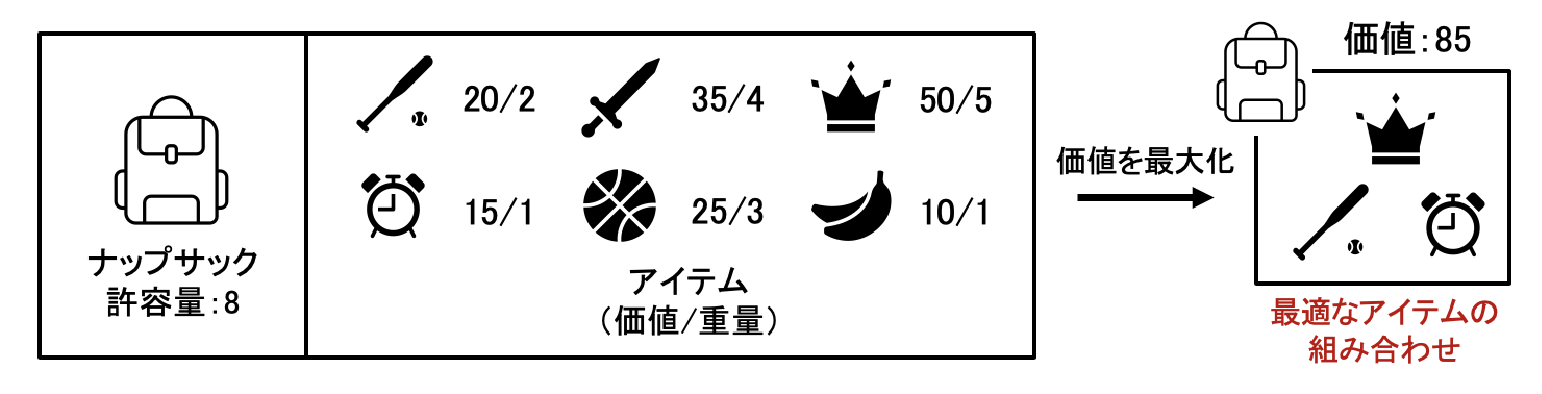
\includegraphics[width=0.9\linewidth]{fig/knapsack.eps}
\caption{ナップサック問題例}
\label{fig:knapsack}
\end{center}
\end{figure}


\subsubsection{定式化}
本章では,RQ1の分析結果をナップサック問題に適用することで,変更提案の選択手法を定式化する.定式化にあたって,ナップサック問題におけるアイテム,アイテムの重量,アイテムの価値,ナップサックの許容量を定義する.

\begin{enumerate}
  \item{\textbf{アイテム:}}
  選択時点において存在している変更提案の中から最適な変更提案の組み合わせを選択するため,\textgt{選択時点において存在している変更提案}を,本手法におけるアイテムと定義する.
  \item{\textbf{アイテムの重量:}}
  コードレビューにおいて,ソースコードの変更規模が大きいものほどレビューに時間がかかると考えられる.そのため,ソースコードの変更規模としてよく用いられる指標である\textgt{変更行数}\cite{diff}を,本手法におけるアイテムの重量と定義する.
  \item{\textbf{アイテムの価値:}}  
  RQ1の予測モデルを用い,\textgt{直近のバージョンリリースに導入される確率}を,本手法におけるアイテムの価値と定義する.
  \item{\textbf{ナップサックの許容量:}}
  アイテムの重量を考慮し,プロジェクトが一定期間でコードレビューできる変更行数を本手法における許容量とする.また,曜日によって作業量に差異が生じる可能性を排除するため,本手法では一定期間として1週間を採用する.よって,\textgt{プロジェクトが1週間でコードレビューできる変更行数}を,本手法におけるナップサックの許容量と定義する.
\end{enumerate}


\subsubsection{分析方法}
本手法が変更提案の選択に有効か否かを分析するために,本手法に基づいて選択された変更提案と,実際の開発においてコードレビューが行われた変更提案を比較する.具体的には,分析対象バージョンがリリースされる1週間前,2週間前,1ヶ月前,2ヶ月前の時点で,その時点から1週間でコードレビューを行う変更提案を本手法によって選択する.選択した変更提案と実際にコードレビューが行われた変更提案の直近のバージョンリリースへの導入数を比較する.

\subsection{選択結果}
各プロジェクトごとに選択した変更提案と実際にコードレビューが行われた変更提案の直近のバージョンリリースへの導入数を比較する.本論文では,選択結果の妥当性を担保するために,15種類の分析対象バージョンの中から直近3バージョンにおいて分析を行う.また,分析を行う際の訓練データとして,各プロジェクトの分析対象バージョン以前にリリースされたバージョンの変更提案を用いる.

\subsubsection{Neutronプロジェクト}\label{chap:neutron}
選択結果を表\ref{table:neutron}に示す.リリース1週間前時点では,2種類の分析対象バージョンにおいて,選択手法によって選択された変更提案の中で直近のバージョンで導入された変更提案数(選択導入提案数)が,実際の開発でコードレビューされた変更提案の中で直近のバージョンで導入された変更提案数(検証導入提案数)を上回り,1種類の分析対象バージョンにおいて下回った.一方,他の分析時点では,全ての分析対象バージョンにおいて選択導入提案数が検証導入提案数を上回った.また,選択手法は直近のバージョンで導入される変更提案のうち,47\%〜100\%の変更提案を選択した.

\begin{table}[t]
  \caption{Neutronプロジェクトにおける選択結果}
    \scalebox{0.63}{
  \label{table:neutron}
  \centering
 \begin{tabular}{l|l|r|r|r|r} \hline
   \multicolumn{1}{c|}{分析時点} & \multicolumn{1}{|c|}{分析対象バージョン} & \multicolumn{1}{|c|}{変更提案数} & \multicolumn{1}{|c}{導入提案数} & \multicolumn{1}{|c|}{選択導入提案数} & \multicolumn{1}{|c}{検証導入提案数} \\ \hline \hline
    & 15.0.0.0b1 & 998 & 16 & 15 & 9 \\ \cline{2-6}
   1週間前 & 19.0.0.0rc1 & 963 & 6 & 5 & 4 \\ \cline{2-6}
    & 20.0.0.0rc1 & 938 & 6 & 5 & 6 \\ \hline
    & 15.0.0.0b1 & 994 & 16 & 15 & 13 \\ \cline{2-6}
   2週間前 & 19.0.0.0rc1 & 973 & 25 & 25 & 14 \\ \cline{2-6}
    & 20.0.0.0rc1 & 944 & 15 & 15 & 12 \\ \hline
    & 15.0.0.0b1 & 990 & 17 & 8 & 7 \\ \cline{2-6}
   1ヶ月前 & 19.0.0.0rc1 & 972 & 25 & 25 & 16 \\ \cline{2-6}
    & 20.0.0.0rc1 & 950 & 25 & 24 & 16 \\ \hline
    & 15.0.0.0b1 & 996 & 31 & 28 & 14 \\ \cline{2-6}
   2ヶ月前 & 19.0.0.0rc1 & 949 & 28 & 21 & 16 \\ \cline{2-6}
    & 20.0.0.0rc1 & 990 & 56 & 53 & 34 \\ \hline
 \end{tabular}
 }


  \caption{Keystoneプロジェクトにおける選択結果}
  \label{table:keystone}
  \centering
    \scalebox{0.63}{
 \begin{tabular}{l|l|r|r|r|r} \hline
   \multicolumn{1}{c|}{分析時点} & \multicolumn{1}{|c|}{分析対象バージョン} & \multicolumn{1}{|c|}{変更提案数} & \multicolumn{1}{|c}{導入提案数} & \multicolumn{1}{|c|}{選択導入提案数} & \multicolumn{1}{|c}{検証導入提案数} \\ \hline \hline
    & 11.0.0.0b1 & 916 & 8 & 5 & 4 \\ \cline{2-6}
   1週間前 & 15.0.0.0rc1 & 917 & 9 & 8 & 8 \\ \cline{2-6}
    & 16.0.0.0rc1 & 890 & 22 & 18 & 17 \\ \hline
    & 11.0.0.0b1 & 924 & 15 & 13 & 12 \\ \cline{2-6}
   2週間前 & 15.0.0.0rc1 & 917 & 11 & 8 & 5 \\ \cline{2-6}
    & 16.0.0.0rc1 & 908 & 39 & 36 & 23 \\ \hline
    & 11.0.0.0b1 & 926 & 22 & 20 & 12 \\ \cline{2-6}
   1ヶ月前 & 15.0.0.0rc1 & 950 & 47 & 42 & 41 \\ \cline{2-6}
    & 16.0.0.0rc1 & 913 & 41 & 18 & 6 \\ \hline
    & 11.0.0.0b1 & 924 & 15 & 13 & 12 \\ \cline{2-6}
   2ヶ月前 & 15.0.0.0rc1 & 917 & 11 & 8 & 5 \\ \cline{2-6}
    & 16.0.0.0rc1 & 908 & 39 & 36 & 23 \\ \hline
 \end{tabular}
 }

  \caption{Horizonプロジェクトにおける選択結果}
  \label{table:horizon}
      \scalebox{0.63}{
  \centering
 \begin{tabular}{l|l|r|r|r|r} \hline
   \multicolumn{1}{c|}{分析時点} & \multicolumn{1}{|c|}{分析対象バージョン} & \multicolumn{1}{|c|}{変更提案数} & \multicolumn{1}{|c}{導入提案数} & \multicolumn{1}{|c|}{選択導入提案数} & \multicolumn{1}{|c}{検証導入提案数} \\ \hline \hline
    & 13.0.0.0b1 & 629 & 20 & 18 & 12 \\ \cline{2-6}
   1週間前 & 14.0.0.0b1 & 649 & 47 & 45 & 27 \\ \cline{2-6}
    & 15.0.0.0b2 & 522 & 18 & 17 & 14 \\ \hline
    & 13.0.0.0b1 & 634 & 11 & 8 & 10 \\ \cline{2-6}
   2週間前 & 14.0.0.0b1 & 603 & 19 & 16 & 17 \\ \cline{2-6}
    & 15.0.0.0b2 & 517 & 7 & 5 & 5 \\ \hline
    & 13.0.0.0b1 & 629 & 20 & 18 & 12 \\ \cline{2-6}
   1ヶ月前 & 14.0.0.0b1 & 649 & 47 & 45 & 27 \\ \cline{2-6}
    & 15.0.0.0b2 & 522 & 18 & 17 & 14 \\ \hline
    & 13.0.0.0b1 & 626 & 29 & 25 & 12 \\ \cline{2-6}
   2ヶ月前 & 14.0.0.0b1 & 660 & 62 & 35 & 21 \\ \cline{2-6}
    & 15.0.0.0b2 & 533 & 21 & 15 & 13 \\ \hline
 \end{tabular}
 }

  \caption{Novaプロジェクトにおける選択結果}
  \label{table:nova}
    \scalebox{0.63}{
      \centering
 \begin{tabular}{l|l|r|r|r|r} \hline
   \multicolumn{1}{c|}{分析時点} & \multicolumn{1}{|c|}{分析対象バージョン} & \multicolumn{1}{|c|}{変更提案数} & \multicolumn{1}{|c}{導入提案数} & \multicolumn{1}{|c|}{選択導入提案数} & \multicolumn{1}{|c}{検証導入提案数} \\ \hline \hline
    & 19.0.0.0rc1 & 3,781 & 9 & 6 & 6 \\ \cline{2-6}
   1週間前 & 21.0.0.0rc1 & 3,355 & 29 & 22 & 24 \\ \cline{2-6}
    & 24.0.0.0rc1 & 3,182 & 6 & 6 & 4 \\ \hline
    & 19.0.0.0rc1 & 3,798 & 24 & 21 & 19 \\ \cline{2-6}
   2週間前 & 21.0.0.0rc1 & 3,402 & 63 & 56 & 37 \\ \cline{2-6}
    & 24.0.0.0rc1 & 3,186 & 9 & 6 & 6 \\ \hline
    & 19.0.0.0rc1 & 3,812 & 90 & 83 & 57 \\ \cline{2-6}
   1ヶ月前 & 21.0.0.0rc1 & 3,415 & 76 & 71 & 39 \\ \cline{2-6}
    & 24.0.0.0rc1 & 3,292 & 104 & 100 & 59 \\ \hline
    & 19.0.0.0rc1 & 3,791 & 118 & 82 & 45 \\ \cline{2-6}
   2ヶ月前 & 21.0.0.0rc1 & 3,488 & 134 & 96 & 26 \\ \cline{2-6}
    & 24.0.0.0rc1 & 3,287 & 83 & 45 & 19 \\ \hline
 \end{tabular}
 }
\end{table}

\subsubsection{Keystoneプロジェクト}\label{chap:keystone}
選択結果を表\ref{table:keystone}に示す.リリース1週間前時点では,2種類の分析対象バージョンにおいて,選択導入提案数が検証導入提案数を上回り,1種類の分析対象バージョンにおいて同数となった.一方,他の分析時点では,全ての分析対象バージョンにおいて選択導入提案数が検証導入提案数を上回った.また,選択手法は直近のバージョンで導入される変更提案のうち,44\%〜92\%の変更提案を選択した.


\subsubsection{Horizonプロジェクト}\label{chap:horizon}
選択結果を表\ref{table:horizon}に示す.リリース2週間前時点では,2種類のバージョンにおいて,選択導入提案数が検証導入提案数を下回り,1種類のバージョンにおいて同数となった.一方,他の分析時点では,全ての分析対象バージョンにおいて選択導入提案数が検証導入提案数を上回った.また,選択手法は直近のバージョンで導入される変更提案のうち,56\%〜96\%の変更提案を選択した.



\subsubsection{Novaプロジェクト}\label{chap:nova}
選択結果を表\ref{table:nova}に示す.リリース1週間前時点では,1種類のバージョンにおいて,選択導入提案数が検証導入提案数を下回り,1種類のバージョンにおいて,選択導入提案数が検証導入提案数を上回り,1種類のバージョンにおいて同数となった.リリース2週間前時点では,2種類のバージョンにおいて,選択導入提案数が検証導入提案数を上回り,1種類のバージョンにおいて同数となった.一方,他の分析時点では,全ての分析対象バージョンにおいて選択導入提案数が検証導入提案数を上回った.また,選択手法は直近のバージョンで導入される変更提案のうち,54\%〜100\%の変更提案を選択した.



\subsection{まとめ}
\ref{chap:neutron}節から\ref{chap:nova}節までの結果についてまとめる.比較的バージョンリリースが遠いリリース1,2ヶ月前の時点においては,全てのプロジェクトの分析対象バージョンにおいて選択導入提案数が検証導入提案数を上回り,選択手法は直近のバージョンで導入される変更提案のうち,44\%〜100\%の変更提案を選択した.また,比較的バージョンリリースが近いリリース1,2週間前の時点においては,全てのプロジェクトにおいて,選択導入提案数が検証導入提案数を下回るもしくは同数となる分析時点が存在し,選択手法は直近のバージョンで導入される変更提案のうち,63\%〜100\%の変更提案を選択した.

%%%%%%%%%%%%%%%%
\section{考察}\label{chap:disc}
%%%%%%%%%%%%%%%%

RQ1の結果から,直近のバージョンリリースに導入される変更提案の予測において,経過時間とレビュー経過時間が変更提案の特徴として重要な説明変数であることがわかり,直近のバージョンリリースに導入される変更提案はバージョンリリースが近くなるにつれて,経過時間,レビュー経過時間ともに短くなることがわかった.また,経過時間,レビュー経過時間の重要度の平均は,リリース2週間前までの時点においてはレビュー経過時間の方が高く,リリース1週間前の時点においては経過時間の方が高くなることがわかった.これらの結果から,リリースまで時間がある場合はコードレビューされてから時間の経っていない変更提案が導入され,リリースまで時間がない場合はコードレビューの有無に関わらず提出されてから時間の経っていない変更提案が導入されると考えられる.

RQ2の結果から,提案手法は,比較的バージョンリリースが遠い時点では,実際の開発より多くの直近のバージョンで導入される変更提案を選択した.一方,バージョンリリースが近い時点では,全プロジェクトにおいて実際の開発の方が多くの直近のバージョンで導入される変更提案を選択した分析時点が存在した.このことから,バージョンリリースが近い時点では,提案手法によって導入されると予測できない変更提案の特徴が導入に関与していることが示唆される.

\subsection{妥当性の脅威}

\subsubsection{内的妥当性}
本研究では,変更提案の予測モデルを構築するために,変更提案から16種類の特徴量を学習させた.RQの結果として決定係数の精度が低かったため,予測のための特徴量の妥当性が危ぶまれる.しかし,本研究では予測モデルによって予測する目的変数の正例と負例の割合は,1:30〜150程度とかなり負例の多いデータセットとなっている.そこで,学習させるデータセットとテストを行うデータセット両方の正例と負例の割合を1:1にして予測したところ,ほとんどの予測タイミングにおいて,決定係数が0.5以上という精度の高い結果が得られた.この結果をもって,予測のための特徴量の妥当性の脅威を削減する.

\subsubsection{外的妥当性}
本研究では,4つのOSSプロジェクトを対象として分析を行なったため,対象とするプロジェクトを変更することで,異なる結果となる可能性がある.本研究では,多くの変更提案が提出されており,かつ現在も開発が続けられているプロジェクトを選択することで,脅威を削減する.

%%%%%%%%%%%%%%%%
\section{おわりに}\label{chap:fig-tab-exp}
%%%%%%%%%%%%%%%%

本論文では,直近のバージョンリリースに導入される変更提案の選択を容易にすることを目的として,開発状況を考慮した変更提案の選択手法を提案し,設定したRQを検証した.対象データセットとして,OpenStackにおけるプロジェクトの中から,膨大な変更提案が提出されているNeutron,Keystone,Horizon,Novaプロジェクトの変更提案を収集し,変更提案の特徴量を学習させることで,直近のバージョンリリースに導入される変更提案の予測モデルを構築した.モデルの予測精度を評価した結果,MAEやRMSEが高い精度であった一方,決定係数の値は低くなるという結果が得られた.また,予測の際に重要となった特徴を確認した結果,リリースが遠い時点では初回のレビューからの経過時間が重要となるが,リリースが近づくにつれて作成からの経過時間が重要となった.


\begin{acknowledgment}
ほげ
\end{acknowledgment}

\bibliographystyle{ipsjunsrt}
\bibliography{bibfile}
\end{document}
